%
%   This file is part of the APS files in the REVTeX 4.1 distribution.
%   Version 4.1r of REVTeX, August 2010
%
%   Copyright (c) 2009, 2010 The American Physical Society.
%
%   See the REVTeX 4 README file for restrictions and more information.
%
\documentclass[%
 reprint,
%superscriptaddress,
%groupedaddress,
%unsortedaddress,
%runinaddress,
%frontmatterverbose, 
% preprint,
%showpacs,preprintnumbers,
%nofootinbib,
%nobibnotes,
%bibnotes,
 amsmath,amssymb,
 aps,
 pra,
%prb,
%rmp,
%prstab,
%prstper,
%floatfix,
]{revtex4-1}

%%%%%%%%%%%%%%%%%%%%%%%%%%%%%%%%%%%%%%%%%%%%%
% IMPORTS
\usepackage{graphicx}          % Include figure files
\usepackage{dcolumn}           % Align table columns on decimal point
\usepackage{bm}                % bold math
% \usepackage{hyperref}          % add hypertext capabilities
% \usepackage[mathlines]{lineno} % Enable numbering of text and display math
% \linenumbers\relax             % Commence numbering lines

\usepackage{lmodern}           % Font package
\usepackage{floatrow}
\usepackage{subfig}
% Non-standard geometry import
%\usepackage[showframe,%Uncomment any one of the following lines to test 
%%scale=0.7, marginratio={1:1, 2:3}, ignoreall,% default settings
%%text={7in,10in},centering,
%%margin=1.5in,
%%total={6.5in,8.75in}, top=1.2in, left=0.9in, includefoot,
%%height=10in,a5paper,hmargin={3cm,0.8in},
%]{geometry}

%%%%%%%%%%%%%%%%%%%%%%%%%%%%%%%%%%%%%%%%%%%%%
% COMMANDS
\newcommand{\D}{\mathrm{d}}
\newcommand{\iu}{{i\mkern1mu}}

%%%%%%%%%%%%%%%%%%%%%%%%%%%%%%%%%%%%%%%%%%%%%
% DOCUMENT
\begin{document}
{\fontfamily{lmss}\selectfont

\preprint{APS/123-QED}

\title{Telescope Diffraction}

\author{Patrick Anker}
\author{Kaitlyn Morrell}
\affiliation{%
 New York University
}

\date{December 17, 2017}

\begin{abstract}
%Abstract *rough* draft
The wave nature of light gives rise to phenomena such as interference and diffraction. These are observed in the application of optics to telescopes. To explore the various effects that result from different telescope designs, we employ two-dimensional Fourier analysis and simulate environmental factors using Gaussian random fields. Additionally, we investigate the results for different power spectrum inputs and examine the effects on the point spread function.
\end{abstract}

\maketitle

%\tableofcontents

\section{\label{sec:intro}Introduction}

Telescopes depend on light from distant sources, which is evident in the word itself: ``tele'' for ``long'' and ``scope'' for ``sight.'' In the realm of ray optics, all light travels as straight lines emanating from point sources. For our purposes, light incident on telescopes from distant stars can be approximated as parallel lines tangent to the aperture of the telescope.

This straight-line approximation breaks down once we consider the effects of the wave-like nature of light. If light were just straight lines, no diffraction patterns would exist. and thus this entire paper would be pointless. However, this is not the case. As the parallel light hits the telescope, most of the light passes by the aperture entrance while some enters the telescope to be recorded. Light upon the boundary of the telescope diffracts since it scatters, and this scattering creates a diffraction pattern that is inherent to the construction of the telescope.

In this paper, we study various telescope construction styles and their innate diffraction patterns. Analyzing these patterns is essential to accurately render the image that the telescope actually sees as opposed to the image that includes the artifacts of the telescope itself.

\section{\label{sec:aperture-psf}Relation of Aperture to Point Spread Function}

Modeling the light that enters the aperture is pretty straightforward. If we consider a simple plane wave like \[f(r)=\tilde{A}e^{\iu kr}\] once the wave hits the telescope, only some of the wave enters the aperture while some does not. This means that the complex amplitude $\tilde{A}$ changes to reflect the filtration incident on the aperture. This adjusted plane wave is the ``Pupil Function'':
\begin{equation}
  P(r, \phi)\exp(-\iu k W(r, \phi)) \label{eq:pupilFunc}
\end{equation}
where $P(r,\phi)$ is some mathematical function that models the cross section of the telescope's aperture, and $W(r, \phi)$ models any induced phase shifts caused by the optics.

While this function on its own is not particularly informative, its Fourier transform, called the \textit{Point Spread Function} (PSF), shows how responsive the telescope is to certain frequencies of light. With this information, a deconvolution of the input image with the PSF produces what the actual input image was.

\subsection{Simple Aperture} \label{subsec:simple-aperture}

The simplest way to model a telescope is with a simple circle:
\begin{align*}
  P(r, \phi) = \bigg\lbrace\begin{array}{c}
  	1,\;\;r \leq R \\ 
    0,\;\; r > R
  \end{array}
\end{align*}
where $R$ is the radius of the telescope. Furthermore, we assume there are no phase shifts in the incident light. This means that the complex exponential in the pupil function evaluates to 1.

\begin{figure}[h!]
  \centering
    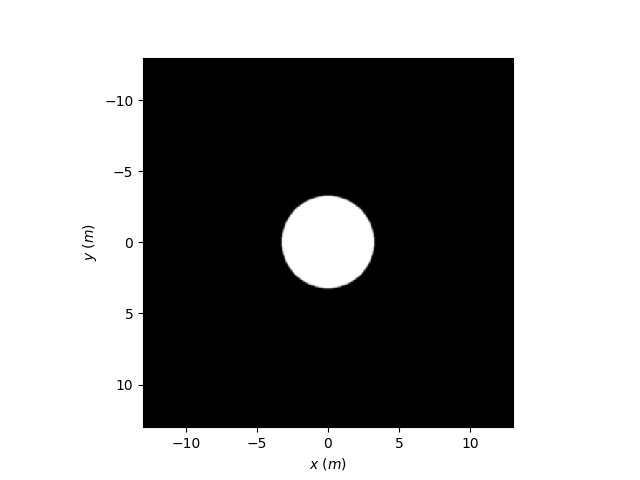
\includegraphics[scale=0.45]{simplepupil.png}
  \caption{The simplest pupil function, a circle}
  \label{fig:simplepupil}
\end{figure}

The reality of the discreteness of computers presents a problem when considering this simple pupil. Since the pixel luminance value is either 0 or 1 in the function, the edges of the circle are jagged. This produces FFT alias artifacts in the PSF, damaging our data. To resolve this, we used a Gaussian filter with standard deviation $\sigma = 1$; this filtering is shown in Fig. \ref{fig:simplepupil} with the soft edges on the circle. Furthermore, to ensure that the FFT would not cause aliasing issues, we padded our image with $\sim$1 diameter of the aperture on either side; a padding scale of $1.183$ diameters had the best results overall for each PSF.

Analytically, the Fourier transform of this pupil function is an example of the 2D polar Fourier transform. Generally, the 2D Fourier transform is of the form:
\begin{equation}
  F(k_x, k_y) = \frac{1}{2\pi}\int\D A\ f(x, y)\exp\left[-\iu(k_x x + k_y y)\right] \label{eq:2dfourier}
\end{equation}
If we perform these transformations:
\begin{align*}
  x &= r\cos\phi & k_x &= k\cos\psi \\
  y &= r\sin\phi & k_y &= k\sin\psi
\end{align*}
then the 2D Fourier transform turns into:
\begin{equation}
  F(k, \psi) = \frac{1}{2\pi}\int\D A\ f(r, \phi)\exp\left[-\iu kr(\cos(\phi - \psi))\right] \label{eq:2dpolarfourier}
\end{equation}
In the special situation where the function $f$ has rotational symmetry, i.e. $f=f(r)$, the integral simplifies to a 1D integral in $r$:
\begin{equation}
  F(k) = \int_0^{\infty}\D r\ r f(r)J_0(kr) \label{eq:2dpolarfouriersym}
\end{equation}
where $J_0$ is the zeroth order of the Bessel function of the first kind. This is the particular integral we care about; the circular aperture obviously has rotational symmetry and has well defined limits: 0 to $R$. Therefore, this integral evaluates to
\begin{equation*}
  F(k) = \frac{R}{k}J_1(R k)
\end{equation*}
However, since the luminance information in an image is only characterized by the intensity, we must take the square of this function to find the desired PSF:
\begin{equation}
  PSF_{\text{simp}}(k) = R^2 \left(\frac{J_1(R k)}{k}\right)^2 \label{eq:psf-simp}
\end{equation}
This particular function generates the \textit{Airy pattern}, a set of concentric circles decaying in luminosity.

\begin{figure}[!ht]
  \centering
    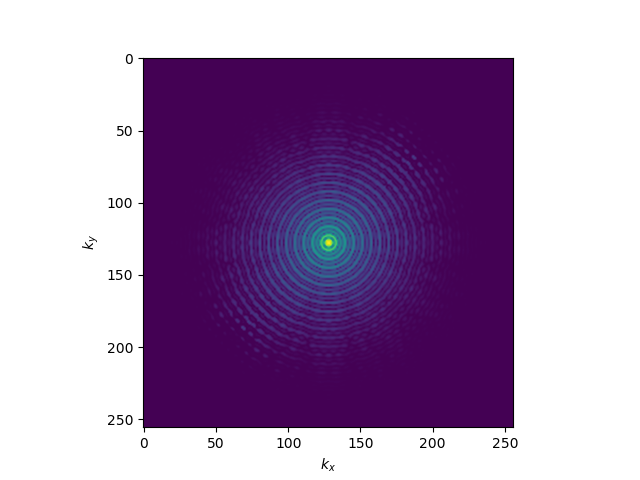
\includegraphics[scale=.45]{simplepsf.png}
  \caption{The computed PSF of the circular aperture}
  \label{fig:simplepsf}
\end{figure}

Using $N=256$ samples per each axis ($x$ and $y$), we performed an FFT on the Gaussian-filtered circular pupil function which produced the image in Fig. \ref{fig:simplepsf}. The ringing and decaying pattern matches what we expected from the theoretical model!

We now use this model to observe how the size of the point spread function varies with aperture size. As shown in Figure~\ref{fig:psfcomp}, the psf size is inversely proportional to aperture size.
\thisfloatsetup{style=plain,subcapbesideposition=top}
\begin{figure}[h!]
\begin{minipage}{.45\textwidth}
  \centering
    \sidesubfloat[]{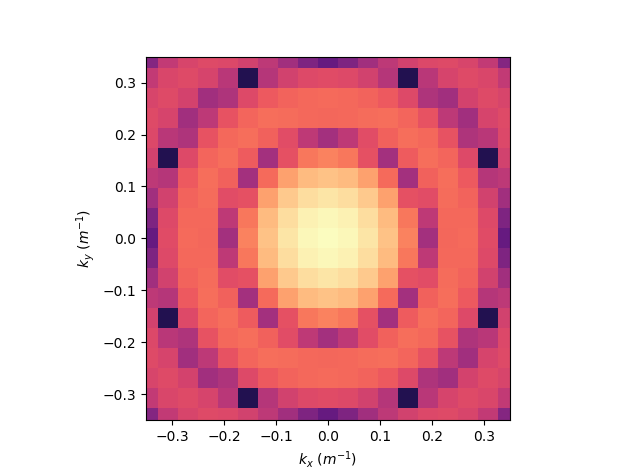
\includegraphics[scale=.25]{simplepsf_6_5.png}\label{fig:6_5}}
\end{minipage}
\begin{minipage}{.45\textwidth}
  \centering
    \sidesubfloat[]{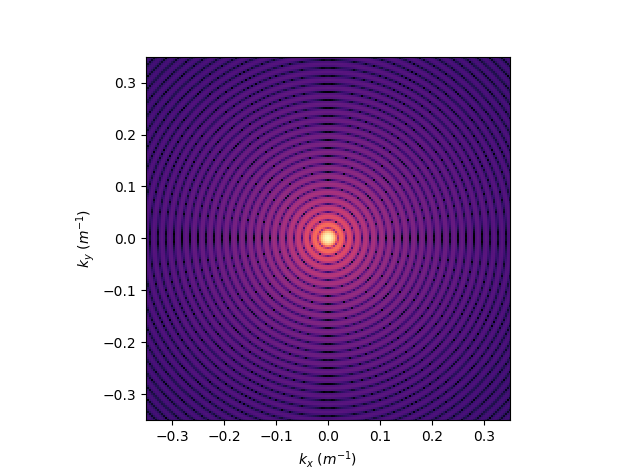
\includegraphics[scale=.25]{simplepsf_65.png}\label{fig:65}}
\end{minipage}

\begin{minipage}{\textwidth}
  \centering
    \sidesubfloat[]{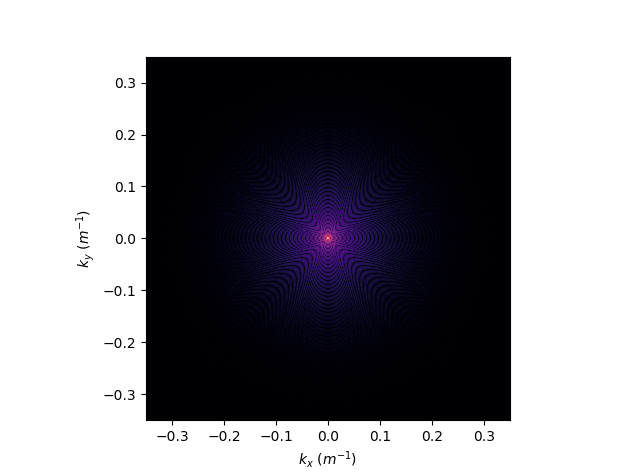
\includegraphics[scale=.25]{simplepsf_650.png}\label{fig:650}}
\end{minipage}
\caption{Comparison of psf size for aperture sizes a) $d=6.5m$, b) $d=65m$, c) $d=650m$}
\label{fig:psfcomp}
\end{figure}


\subsection{Cassegrain Aperture} \label{subsec:cassegrain-aperture}

Most modern telescopes today are derived from the Cassegrain structure wherein the light incident on the aperture is reflected onto a secondary mirror in the middle of the aperture, which then reflects the light to the focal point (see Fig. \ref{fig:cassegrain-schem}).

\begin{figure}[!ht]
  \centering
  	\includegraphics[scale=.45]{casse.png}
  \caption{Cassegrain reflector schematic (https://goo.gl/4mJ1YF, CC BY-SA 4.0 License)}
  \label{fig:cassegrain-schem}
\end{figure}

This hyperbolic secondary mirror affects the simple pupil function by superimposing a ``negative'' circle centered at the origin. This creates a donut, with the mathematical description
% 
\begin{align*}
  P(r, \phi) = \bigg\lbrace\begin{array}{c}
  	1,\;\;r \leq R_1 \\ 
    0,\;\; r > R_1
  \end{array} - \bigg\lbrace\begin{array}{c}
  	1,\;\;r \leq R_0 \\ 
    0,\;\; r > R_0
  \end{array}
\end{align*}
where $R_0$ is the inner radius and $R_1$ is the outer radius. As the Fourier transform is a linear operator, the PSF for the Cassegrain pupil is the squared amplitude of a superposition of one simple pupil and another simple pupil with a smaller radius. Using Eq. \ref{eq:2dpolarfouriersym}, we can swap $f(r)$ for our piecewise defined Cassegrain pupil $P(r, \phi)$ to show that the Cassegrain PSF is indeed related to a superposition of two simple pupils:
% 
\begin{align*}
    F(k) &= \int_0^{\infty}\D r\ r f(r)J_0(kr) \\
         &= \int_0^{R_1}\D r\ rJ_0(kr) - \int_0^{R_0}\D r\ rJ_0(kr) \\
         &= \frac{R_1}{k}J_1(R_1 k) - \frac{R_0}{k}J_1(R_0 k) \\
         &= \frac{1}{k}\left(R_1J_1(R_1 k) - R_0J_1(R_0 k)\right) \\
         &\Downarrow \\
    PSF_{\text{casse}}(k) &= F^*(k)F(k) \\
                          &= \frac{1}{k^2}\left(R_1J_1(R_1 k) - R_0J_1(R_0 k)\right)^2
\end{align*}

Actually rendering a Cassegrain design suffered similar issues that the simple pupil had regarding roughness. Without the Gaussian filtering, the rough edges in the Cassegrain PSF created noise in the high modes which caused FFT aliasing and mirroring (see Fig. \ref{fig:cassepsf-noise}).
% 
\thisfloatsetup{style=plain,subcapbesideposition=top}
\begin{figure}[!ht]
   \begin{minipage}{.45\textwidth}
      \centering
        \sidesubfloat[]{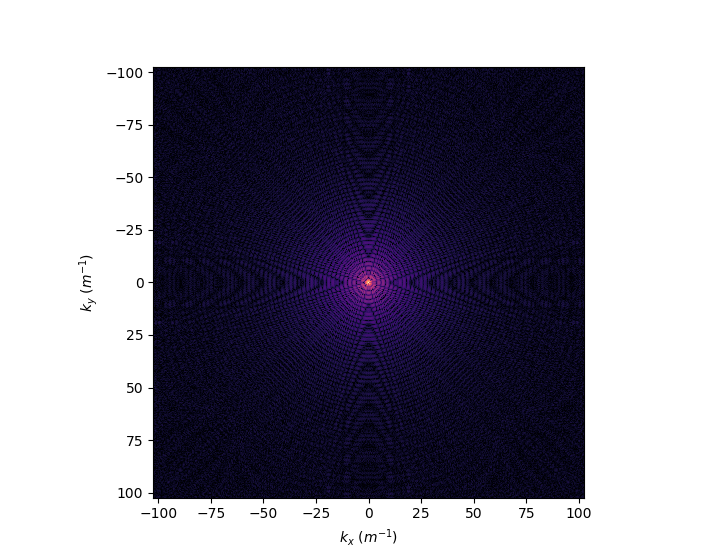
\includegraphics[scale=.20]{cassepsf-noise.png}}
    \end{minipage}
    \begin{minipage}{.45\textwidth}
      \centering
        \sidesubfloat[]{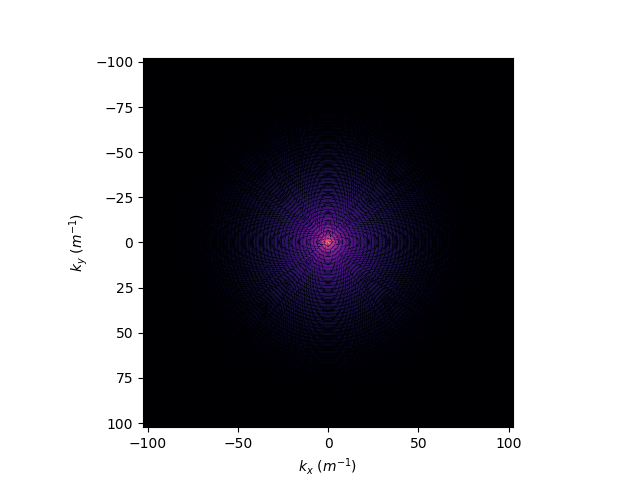
\includegraphics[scale=.20]{cassepsf-clean.png}}
    \end{minipage}
    
    \begin{minipage}{.45\textwidth}
      \centering
        \sidesubfloat[]{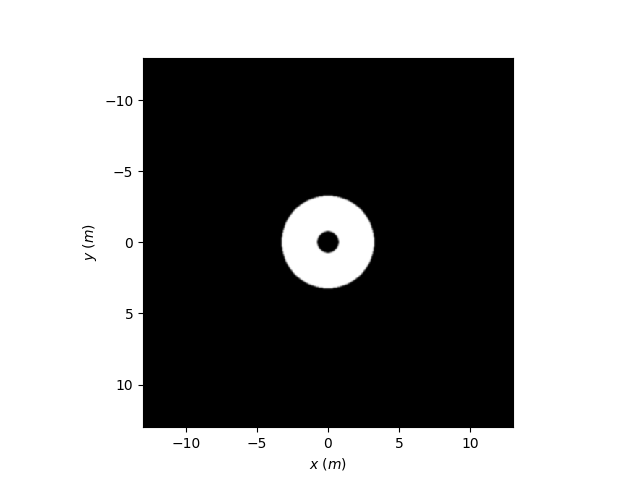
\includegraphics[scale=.20]{cassepupil.png}}
    \end{minipage}
    \caption{In (a), no Gaussian filtering is used; in (b), Gaussian filtering is used. The pupil in question is (c).}
    \label{fig:cassepsf-noise}
\end{figure}

\subsection{Actual Telescope Construction} \label{subsec:actual-aperture}

Physically, there is no such thing as a floating mirror as the mathematically pure Cassegrain pupil shows. Instead, to install this mirror, some struts are needed to hold the secondary mirror in place. The presence of the struts create diffraction patterns known as ``diffraction spikes.'' These spikes are present in our day to day life within our own eyes. If one ever looks directly at a point source of light -- say a street lamp -- the light appears to be ``star'' shaped. The ``star'' pattern is actually a result of light diffracting off of blood vessels in our eyes.

\begin{figure}[!ht]
    \centering
        \includegraphics[scale=0.43]{wispy.png}
    \caption{``Wispy Remains of Supernova Explosion Hide Possible Survivor'' from the Hubble Space Telescope}
    \label{fig:wispy}
\end{figure}

The same situation is present in diffraction-limited telescopes, like land-based optical telescopes and space observatories like the Hubble Telescope. The spikes around stars in Fig. \ref{fig:wispy} are inherent to the struts in the telescope. Specifically, the secondary mirror in the Hubble telescope is enclosed in a baffle structure attached to the barrel with four struts, corresponding to the four spikes.

\begin{figure}[!ht]
    \centering
        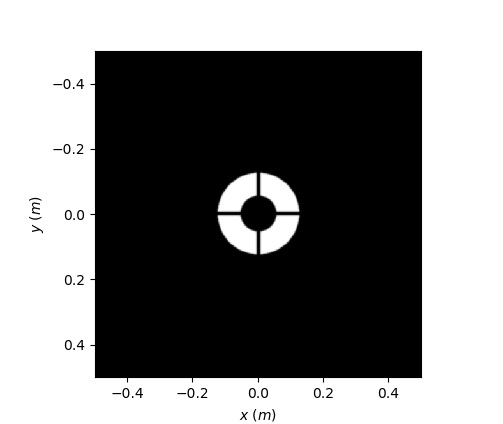
\includegraphics[scale=0.43]{modelpupil.png}
    \caption{Our model's pupil function with \textit{no} turbulence modeled}
    \label{fig:modelpupil}
\end{figure}

Modeling these four spikes was rather straightforward. For the rest of this paper, we are considering our model of an Orion $f/8$ 10" Cassegrain telescope which includes an aperture of 250$mm$, a secondary mirror with diameter 110$mm$, and four struts. The pupil, in Fig. \ref{fig:modelpupil}, is much like the Cassegrain pupil in that it has the donut pattern. However, the simple Airy pattern gets a major additional artifact: the diffraction spikes!

\begin{figure}[!ht]
    \centering
    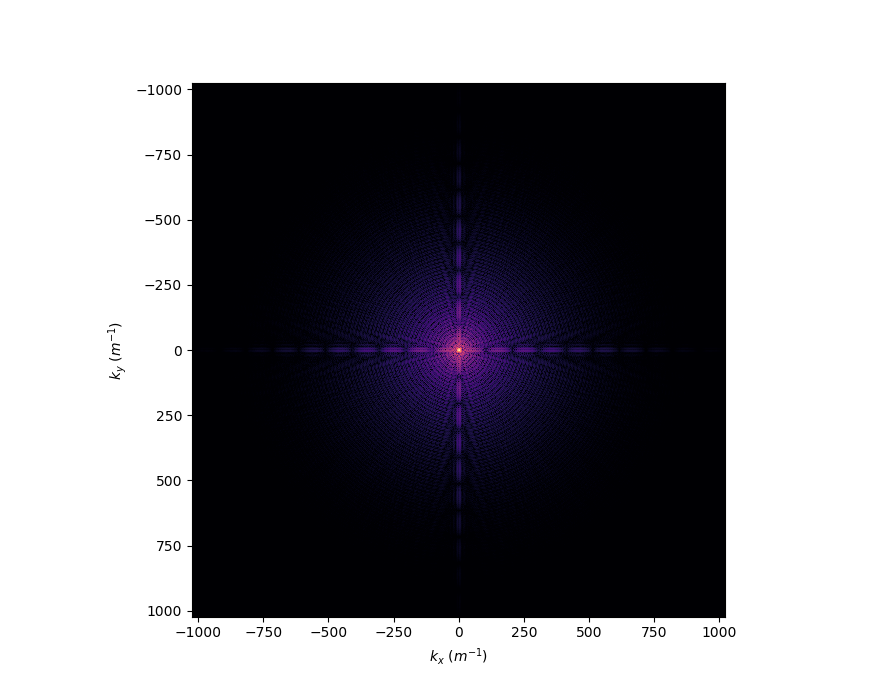
\includegraphics[scale=0.4]{modeltpsf.png}
    \caption{Our model's PSF using $\lambda = 550nm$ light without atmospheric turbulence}
    \label{fig:modelpsf-no-turb}
\end{figure}

Fig. \ref{fig:modelpsf-no-turb} shows what happens when monochromatic light is incident on the optics: diffraction spikes with nodes radiate along the axes while the Cassegrain Airy pattern underlies the entire structure. These nodes are actually depedent on the wavelength of light used. If a continuous spectrum of light were incident on the optics, the nodes would ultimately disappear due to smoothing. At one node may be one wavelength's particular antinode. With 50 wavelengths evenly spaced between $400nm$ and $700nm$, the nodes -- while still present -- begin to fade out, shown in Fig. \ref{fig:modeltcomp}.

\begin{figure}[!ht]
    \centering
        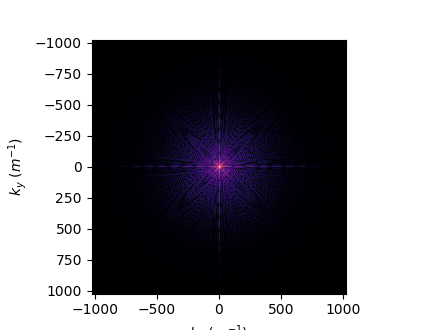
\includegraphics[scale=0.45]{modeltcomp.png}
    \caption{Lessened node presence with 50 sampled visible wavelengths of light}
    \label{fig:modeltcomp}
\end{figure}

\section{The Effects of Environmental Factors on the Point Spread Function} \label{sec:environment}

The phase shift in the complex pupil function (Eq. ~\ref{eq:pupilFunc}) can arise from different environmental factors such as imperfections in the telescope mirror or light-particle interactions in the atmosphere. To analyze how these factors affect the PSF, we simulate the phase shifts using Gaussian random fields scaled by different power spectra corresponding to the different factors.

\subsection{Gaussian Random Field Simulation} \label{subsec:gaussian-fields}
In order to simulate phase shifts from different causes, we have created a function that will generate a Gaussian random field given a power spectrum, $\Phi(\kappa)$. The values in the fields are selected from Gaussian distributions with a mean of zero and a scaling determined by the power spectrum. They are created by selecting an independent Gaussian random value for each Fourier mode in $\vec{\kappa}-$space followed by an inverse FFT back to configuration space. An example of one such field is shown in Figure ~\ref{fig:GaussianRandField}

\begin{figure}[h!]
  \centering
    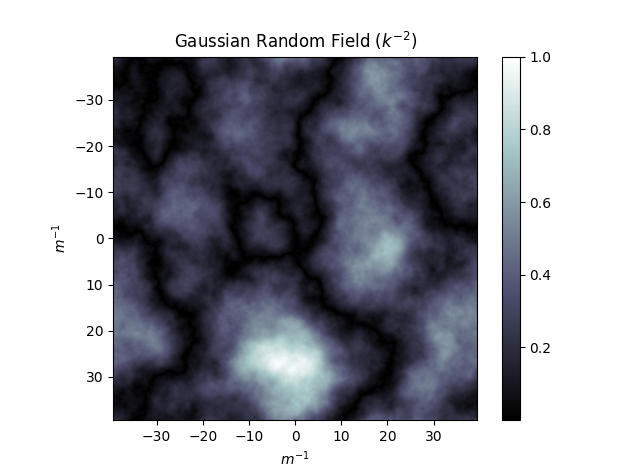
\includegraphics[scale=.45]{gaussrandfield.png}
  \caption{Gaussian Random Field Simulation for $\Phi(\kappa)\propto k^{-2}$}
  \label{fig:GaussianRandField}
\end{figure}

\subsection{Atmospheric Fluctuations} \label{subsec:atmosphere-model}
As a light wave from an astronomical source propagates towards earth through the atmosphere, the initially plane wavefront is perturbed by optical turbulence. Resulting from mixing of layers of air with different temperatures, the turbulence varies constantly. The average shift of the wavefront due to turbulence can be described with the coherence length. 

Since atmospheric turbulent flow is very complex, there are several different models used to evaluate its effects. One model was developed by Andrei Kolmogorov and assumes an initial energy on a large outer scale, $L_0$, that then forms eddies and is eventually dissipated at a small inner scale, $\ell_0$. The Kolmogorov phase power spectrum as a function of spatial frequency $\kappa$ is given by 
\begin{equation}
  \Phi(\kappa) = 0.023r_0^{-5/3}\kappa^{-11/3} \label{eq:kolmogorov}
\end{equation}
where $r_0$ is the Fried parameter, also known as the coherence length, which quantifies the integrated strength of the turbulence.

This model, however, is not valid in the limit of very large and very small scales. We use the Von Karman spectrum which accounts for this and is given by
\begin{equation}
  \Phi(\kappa) = 0.023\frac{|\kappa^2 + \kappa_0^2|^{-11/6}}{r_0^{5/3}}\exp{-\frac{\kappa^2}{\kappa_m^2}} \label{eq:vonkarman}
\end{equation}
where $\kappa_0 = 2\pi/L_0$ and $\kappa_m = 5.92/\ell_0$.

We can see how this turbulence affects the incoming wavefront by looking at the phase shift as a function of spatial frequency in Figure~\ref{fig:GaussATM}.
\begin{figure}[H]
  \centering
    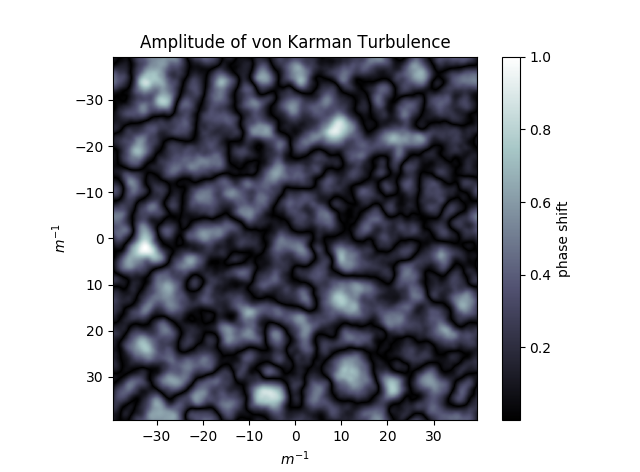
\includegraphics[scale=.4]{gaussatm.png}
  \caption{Phase Shift due to Von Karman Turbulence}
  \label{fig:GaussATM}
\end{figure}

On small spatial scales, the turbulent energy is dissipated, and so the effects on the wavefront are minimal. For the scale of our atmospheric turbulence model, we use a coherence length of $r_0 = 20cm$, an inner scale defined by $\ell_0 = 1 mm$ and an outer scale defined by $L_0 = 20 m$.
\thisfloatsetup{style=plain,subcapbesideposition=top}
\begin{figure}[H]
\begin{minipage}{.45\textwidth}
  \centering
    \sidesubfloat[]{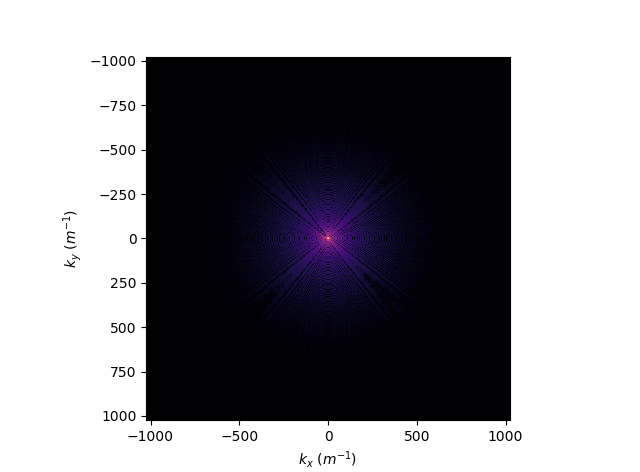
\includegraphics[scale=.24]{simplepsfr.png}\label{fig:greensimp}}
\end{minipage}
\begin{minipage}{.45\textwidth}
  \centering
    \sidesubfloat[]{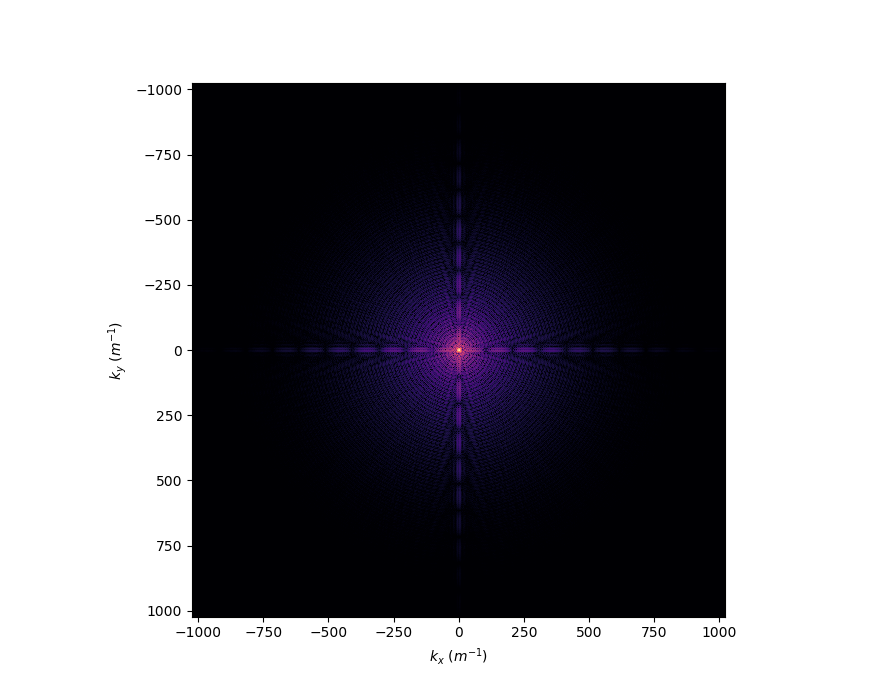
\includegraphics[scale=.16]{modeltpsf.png}\label{fig:greenturbfree}}
\end{minipage}

\begin{minipage}{\textwidth}
  \centering
    \sidesubfloat[]{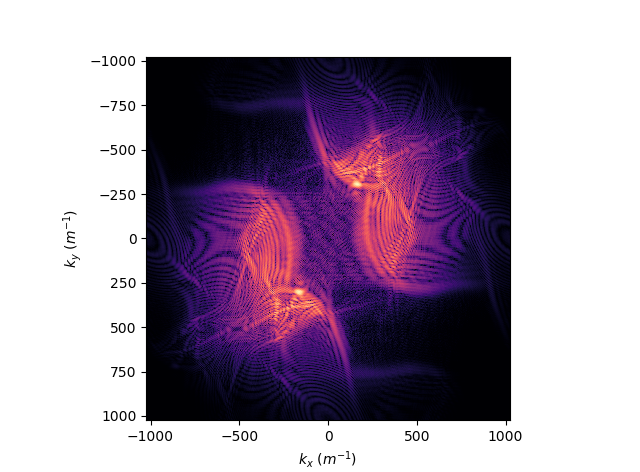
\includegraphics[scale=.24]{modelpsfg.png}\label{fig:greenall}}
\end{minipage}

\caption{Effect of turbulent point spread function on visible light $\lambda=550nm$}
\label{fig:turbeffect}
\end{figure}

Fig. ~\ref{fig:greensimp} shows the point spread function for incoming green light with no atmospheric turbulence and a simple aperture design. Fig. ~\ref{fig:greenturbfree} shows the point spread function for incoming green light with the Cassegrain design with four struts but still no turbulence. Finally, Fig. ~\ref{fig:greenall} shows the point spread function for incoming green light with the atmospheric turbulence added. We can see from this that the effect of the turbulence on the point spread function is to completely obstruct the image for that wavelength of light. If we look at the effect on incoming light across the visible spectrum (range 400nm to 700nm), we see that the turbulence interferes with the full spectrum and the combined effect is a complete, noisy blur of any details originally contained in the image (Fig. \ref{fig:turbvis}).

\begin{figure}[H]
  \centering
    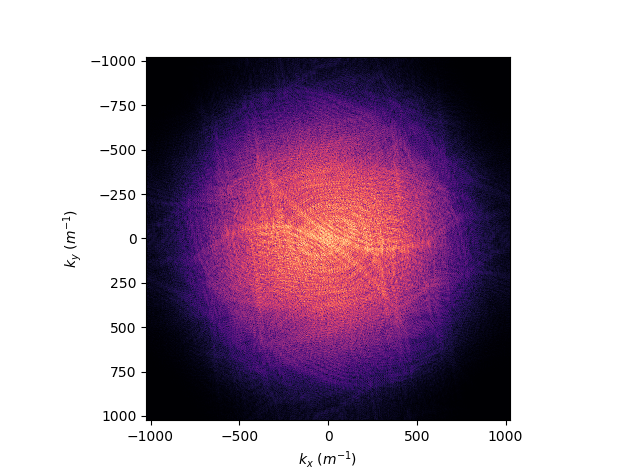
\includegraphics[scale=.35]{modelpsfcomp.png}
\caption{Effect of turbulence on point spread function for visible light spectrum}
\label{fig:turbvis}
\end{figure}

\subsection{Mirror Imperfections} \label{subsec:mirror-issues}
Small imperfections in the mirror can produce phase shifts of correspondingly small wavelengths and are therefore simulated by passing a $\Phi(\kappa)$ with power at large $\kappa$ into our Gaussian random field generating function. These fluctuations are so small in comparison to the fluctuations due to atmospheric turbulence, that they are only noticeable when the turbulence is not present.
\begin{figure}[H]
  \centering
    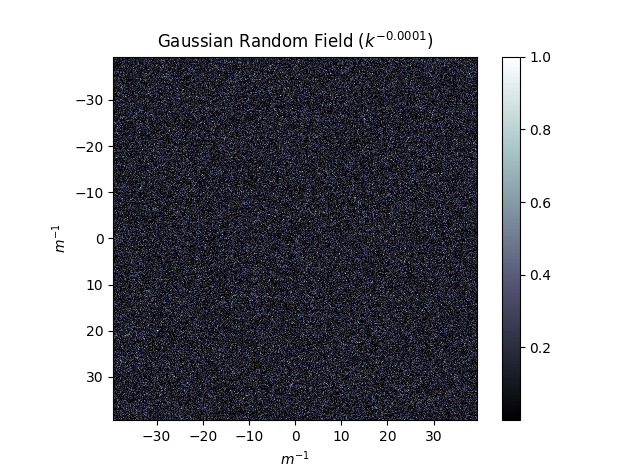
\includegraphics[scale=.35]{gaussmirror.png}
\caption{Gaussian random field for mirror imperfections $\Phi(\kappa)\propto k^{-0.0001} $}
\label{fig:mirror}
\end{figure}

Figure ~\ref{fig:mirror} shows that the phase shifts due to mirror imperfections are very small and lack any structure when compared to the atmospheric turbulence phase shifts. This verifies that shifts due to mirror imperfections will only be a major problem in the absence of atmospheric turbulence.

\begin{thebibliography}{9}
\bibitem{Osborn} Osborn, James. "Profiling the Turbulent Atmosphere and Novel Correction Techniques for Imaging and Photometry in Astronomy." \textit{Durham University}, 2010. %http://community.dur.ac.uk/james.osborn/thesis/thesisse3.html
\bibitem{TeleOptics} Sacek, Vladimir. "Amateur Telescope Optics." \textit{Amateur Telescope Optics}, 14 July 2006, www.telescope-optics.net/. %http://www.telescope-optics.net/induced.htm
\end{thebibliography}

}\end{document}
